\section{Limitations due to SysMLv2 dependence}\label{sec:limitation}
\sideboxbegin{o}
This section presents the limitation encountered while integrating the functionalities of Trace\textit{a} into SysMLv2.
\sideboxend

During this fifth deliverable we ran into the limitations pointed out in the fourth deliverable.
In this section, we present these limitations \ughu{and debrief on the exchange with the SysMLv2 Submission team.} 
 
\subsection{Metadata feature library -- a promising idea}
\begin{figure}[ht]      
	\centering
	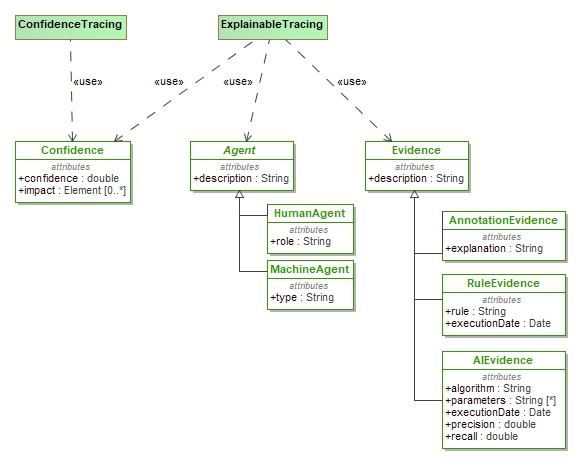
\includegraphics[width=.9\linewidth]{images/explainability-datatype.jpg}
	\caption{Metadatatypes for quality traceability including an assessment of confidence and monitoring of the identification processes used.}
	\label{fig:datatypes}
\end{figure}

% \vspace{3em}
The Listings \ref{lst:featurelibrary1} and \ref{lst:featurelibrary2} present our feature library {in SysML}. Listing~\ref{lst:featurelibrary1} contains the library declaration; Listing~\ref{lst:featurelibrary2} contains an example of application of such datatype  defined on a concrete example. It illustrates the allocation of a confidence value of 0.7 to a connection between a requirement (req) and a package. The second case (line 16 to 20) attributes a description and points to an element impacted (by the evaluation of the confidence),
% \vspace{10cm}

\begin{center}
\begin{lstlisting}[caption={Definition of a datatype dedicated to traceability (partial listing).},
label=lst:featurelibrary1,
style=mystylesysml,
linewidth=15cm,
xleftmargin=2.2cm,
morekeywords={part,filter}]
 package TracingAnnotations {
	attribute def ConfidenceTracing {
		attribute confidence : Real;
		attribute impact : Anything[*]
		assert constraint 
		  { confidence >= 0.0 && confidence <= 1.0 } 
	}
	 
	attribute def ExplainableTracing {
		attribute description : String;
		attribute evidence : Evidence;
		attribute agent : Agent;
	}  
 }
\end{lstlisting}
\end{center}  

\begin{center}
\begin{lstlisting}[caption={Use of metadata features for traceability},
label=lst:featurelibrary2,
style=mystylesysml,
frame=shadowbox,
rulesepcolor=\color{blue},
linewidth=15cm,
xleftmargin=2.2cm,
morekeywords={confidence,description,evidence,impact, part, req,package}]
 import package TracingAnnotations::*;

 /*Definition of the target system. */
 part vehiculetest {}
 req RE01_MLV {}
 package UMLCD_CORE {}

 /*Assignment of a confidence of 0.7 to the Req2Design link.*/
 connection Req2Design connect RE01_MLV to UMLCD_CORE {
   @ConfidenceTracing {
     confidence = 0.7;
   }
 }
 
 /*Assigning a description and an impact to the Req2Design link.*/
 connection Req2Design connect RE01_MLV to UMLCD_CORE {
   @ExplainableTracing {
     description = "Something";
     impact = (vehiculetest);
   }
 }
 
\end{lstlisting}
\end{center}



\subsection{Model level expression -- a deceitful implementation}
\begin{figure}[h]     
	\centering
	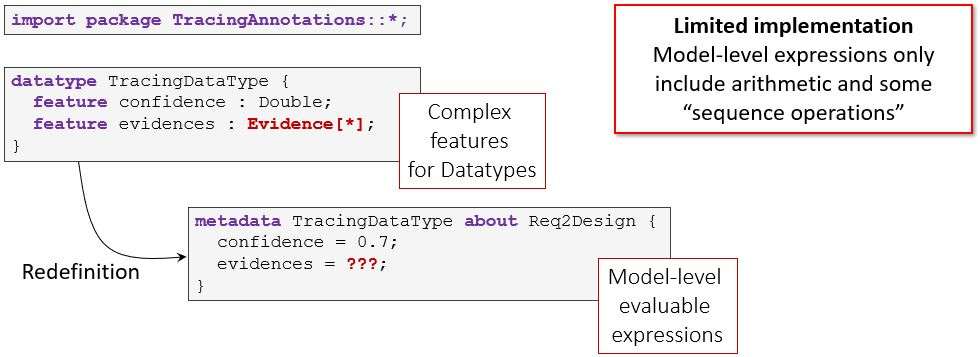
\includegraphics[width=.95\linewidth]{images/strategy4-metadatatype.jpg}
	\caption{Annotations and complex datatypes. }
	\label{fig:metadatatypes}
\end{figure}

\begin{figure}[ht]     
	\centering
	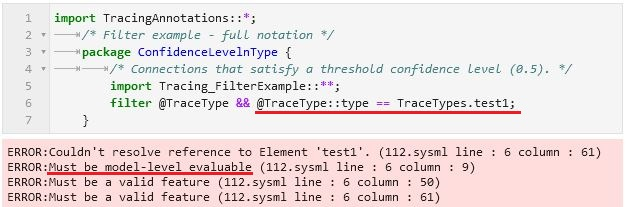
\includegraphics[width=.99\linewidth]{images/viz_filterexample_err.JPG}
	\caption{Limitation of the implementation of model-level evaluable expressions.}
	\label{fig:filtererr}
\end{figure}
To avoid modifying the fundamental elements of {KerML}, our second idea was to redefine an annotation type dedicated to tracing. To do this, a TracingAnnotation links a Relationship to a TracingElement just as an annotation links an Element to an AnnotatingElement. \ugh{.....................................}


% \vspace{6cm}
Nonetheless, the concept of annotation is to be retained here -- it suits perfectly the idea of traceability \textit{orthogonal} to the software. With tracing annotation, a change in the traced elements does not necessarily impact the tracing elements, and vice versa.

\subsection{SysMLv2 Submission Team -- a cordial but interested exchange}